\documentclass[
 reprint,
 twocolumn,
 amsmath,amssymb,
 aps,
 pra,
 floatfix,
]{revtex4-1}

\usepackage{graphicx}% Include figure files
\usepackage{natbib}
\usepackage{hyperref}
\usepackage{listings}
% \usepackage[mathlines]{lineno}% Enable numbering of text and display math

\bibliographystyle{plain}
\graphicspath{ {./img/} }

\begin{document}

\title{Estimating Muon Lifetime}

\author{Stanley Yu (sy2751)}
 \email{stanley.yu@columbia.edu}
\author{Adam He (ash2223)}
 \email{ash2223r@institution.edu}
\affiliation{PHYS 3081 E.K.A. Advanced Physics Laboratory, Columbia University}

\date{March 18, 2020}

\begin{abstract}

To better characterize the behavior of subatomic particles, we estimate the
mean lifetime of muons produced by cosmic rays colliding with particles in
Earth's upper atmosphere. Using 1000 individually collected muon double events
collected over 36 hours and 18 minutes, we find that the mean muon lifetime in
a vacuum is $2.22 \mu s \pm 0.0764 \mu s$. The original muon lifetime
measurement was corrected for the accidental events involving multiple unrelated
events occurring within the same interval and for the bias resulting from the
finite window size. This result is within $.45\%$ of the currently accepted
mean muon lifetime. We also plot a histogram and fit the plot to an exponential
decay model to demonstrate that the distribution of muon lifetimes behaves
exponnentially as expected.

\end{abstract}

\maketitle

\section{Introduction}
Ultrahigh-energy cosmic rays bombard the atoms of oxygen, nitrogen, and other
molecules comprising Earth's atmospheric gases, emitting gamma radiation and
creating an air shower of subatomic particles including muons. Specifically,
a cosmic ray proton colliding with atomic nuclei will typically produce a
secondary proton or neutron alongside other energetic hadrons, mainly pions.
Since pions are unstable, they may decay into other fundamental particles.
Neutral pions immediately decay into two photons, generating an electromagnetic
shower of electron-positron pairs and gamma rays.\cite{gaisser2016} On the other
hand, the fate of charged pions depends on their energy. High-energy charged
pions will interact with more atmospheric particles and create more neutral
pions that propagate the electromagnetic portion of the air shower. Low-energy
charged pions instead decay into muons and muon neutrinos,
which survive to Earth's surface because of time dilation.
\begin{align}
    \pi^+ &= \mu^+ + \nu\\
    \pi^- &= \mu^- + \nu
\end{align}
The muon is an elementary particle classified as a lepton in the Standard Model of particle physics
and possesses a similar charge and spin to the electron but with a mass about 207 times the electron's.\cite{nistconstant}
Without relativity, muons would only survive without decaying a distance of
approximately 456 ($2.197 \mu s * \ln(2) * 0.9997c$) meters (as seen from the Earth). This is only enough to
cover the upper region of the atmosphere, which, in total, spans about 12
kilometers. However, muons are detectable in significant amounts from the
ground and even deep underground, highlighting the penetrative nature of these
particles. Comparing the difference between the number of muons expected from
a Newtonian perspective and that from a relativistic perspective allows for the
determination of the mean muon lifetime $T_0$.
\begin{align}
    M_{Newton} &= e^{-Z/T_0}\\
    M_{relativity} &= e^{-Z/\gamma T_0}
\end{align}
$M$ is the number of muons measured at sea level, while $N$ is the number
measured in the upper atmosphere. $Z$ is the time it takes for a muon to
traverse the distance between the two in the rest frame of the Earth. The
relativistic properties of muons are of great interest to scientists and
were studied closely in the Rossi-Hall experiment (1941). By setting up
detectors at different altitudes on a mountain in Colorado, Bruno Rossi and 
David B. Hall measured the muons' momentum and computed their mean lifetime,
obtaining a proper lifetime of $2.4 \pm 0.3 \mu s$.\cite{PhysRev.59.223} Their
result verified time dilation as predicted by special relativity, an example of
the significant achievements possible through our understanding and application
of muons.

Modern experiments have more precisely determined the mean muon lifetime to be
$2.1969803(2.2) \mu s$ using more than $2 * 10^{12}$ recorded decays.
Such observations were made possible by precisely setting up the proper equipment
to construct a time-structured, low-energy muon beam directed towards a segmented
plastic scintillator array.\cite{PhysRevLett.106.041803} These experiments
capture pions to take advantage of their decay into muons, which are detected
by the scintillator array. With this setup, we can measure the time from some of the
muons' collision with the scintillation material and its subsequent decay into
electrons, neutrinos, and antineutrinos. Then, we can quantify
the number of radioactive particles $N$ left after a given amount of time $t$ by
modeling a familiar exponential distribution:
\begin{align}
    N(t) = N_0 \exp(-\lambda t)
\end{align}
where $N_0$ is the number of unstable particles at $t = 0$. By definition, the
exponential time constant is the reciprocal of the decay rate, $\tau = 1/\lambda$.
Differentiating (5) then gives the rate of decay in terms of the mean lifetime:
\begin{align}
    \frac{dN}{dt} = (\frac{-1}{\tau})N_0\exp(\frac{-t}{\tau})
\end{align}
Taking the expectation of particles decaying according to this exponential
distribution then gives the mean lifetime:
\begin{align}
    E[t] &= \frac{1}{N_0}\int_0^\infty t \frac{dN}{dt} dt\\
    &= (\frac{-1}{\tau})\int_0^\infty t \exp(\frac{-t}{\tau}) dt
\end{align}
Thus, to accurately determine the mean lifetime, we design an experimental
procedure to record the muons' rate of decay and plot a waveform showing the
total time interval from collision to decay, which we can feed into a computer
program to graph and analyze.

\section{Methods}
The experiment's objective is to use a scintillation detector to record the time
interval between the moment the muon enters the detector and the moment it
decays to an electron, among other particles. Although
both muons and antimuons result from cosmic ray showers, we do not distinguish
between the two because their lifetimes in a vacuum are equivalent, and, in air,
the muon lifetime is only slightly shorter than the antimuon lifetime due to
muon capture.

The E.K.A. Laboratory generously provides a detector constructed from a
plastic scintillator and photomultiplier tube. The scintillation detector takes
advantage of the small flash of light known as a scintillation that occurs when
charged particles strike certain materials to produce an electrical pulse
amplified by the photomultiplier tube. It consists of a scintillating material
optically coupled to a photomultiplier via a light guide. The resulting
electrical signal produced from the setup is then fed into other equipment for
analysis. Directly from the detector, the electrical pulse generated by the muon capture
and decay feeds into a discriminator, which filters out low-amplitude noise.
The oscilloscope then allows us to view the resulting signal.

The following discusses additional details about the equipment and their
components: the plastic scintillator, photomultiplier tube, oscilloscope, and
program used for waveform analysis.

\subsection{Plastic Scintillator}

The plastic scintillator attached to the photomultiplier tube is a solution of
organic scintillators in a solid plastic solvent. Organic scintillators are
aromatic hydrocarbon compounds containing linked or condensed benzene-ring
structures. Scintillation light in these compounds arises from transitions made
by the free valence electrons of the molecules. When a muon travels to the
scintillator, the ionization energy from the penetrating radiation excites both
the electron and vibrational levels. When the electron relaxes, it emits a
photon of light, which is guided towards the photomultiplier tube. Plastics
offer an extremely fast signal with a decay constant of about 2-3 ns and a high
light output.\cite{leotechniquesforexperiments}

\subsection{Photomultiplier Tube}

Photomultiplier tubes (PMT) are highly sensitive electron tube devices for
detecting ultraviolet, visible, and infrared light and converting it into a
measurable electric current. The PMT consists of a photocathode made of
photosensitive material, an optical input system with a focusing electrode, a
dynode string that acts as a multiplier, and an anode. It awaits the plastic
scintillator's emission of a photon of light, which causes the photocathode
to emit an electorn via the photoelectric effect. This electron is directed
towards the dynode string, causing an electron cascade that is collected at
the anode to produce a current for measuring and analysis.\cite{leotechniquesforexperiments}

\subsection{Discriminator}

A discriminator is an electornic circuit that responds only to input signals
exceeding a threshold value by producing a standard logic signal. This allows
us to block out low amplitude noise from our detector and act as a simple
analog-to-digital converter for processing by other electronics.

\subsection{LeCroy WaveSurfer 3034z Oscilloscope}

The oscilloscope is an electronic device that visualizes changing signal
voltages as a two-dimensional plot of signal versus time. The LeCroy WaveSurfer
3034z Oscilloscope also presents many options for adjusting the rate and type
of data received. To record the relevant observations, we chose a threshold voltage
of $-1.555$ V and set the interval
trigger to $[200 ns, 10 \mu s]$, with each waveform comprising about 40,000
points, each representing a 2-tuple of time and amplitude. For the background
calculation, we chose an interval trigger of $[20 \mu s, 30 \mu s]$. A diagram
from the LeCroy WaveSurfer 3000z Manual is shown in Figure 1 describing the
range of functionality and adjustments available for our data collection.

\begin{figure}
    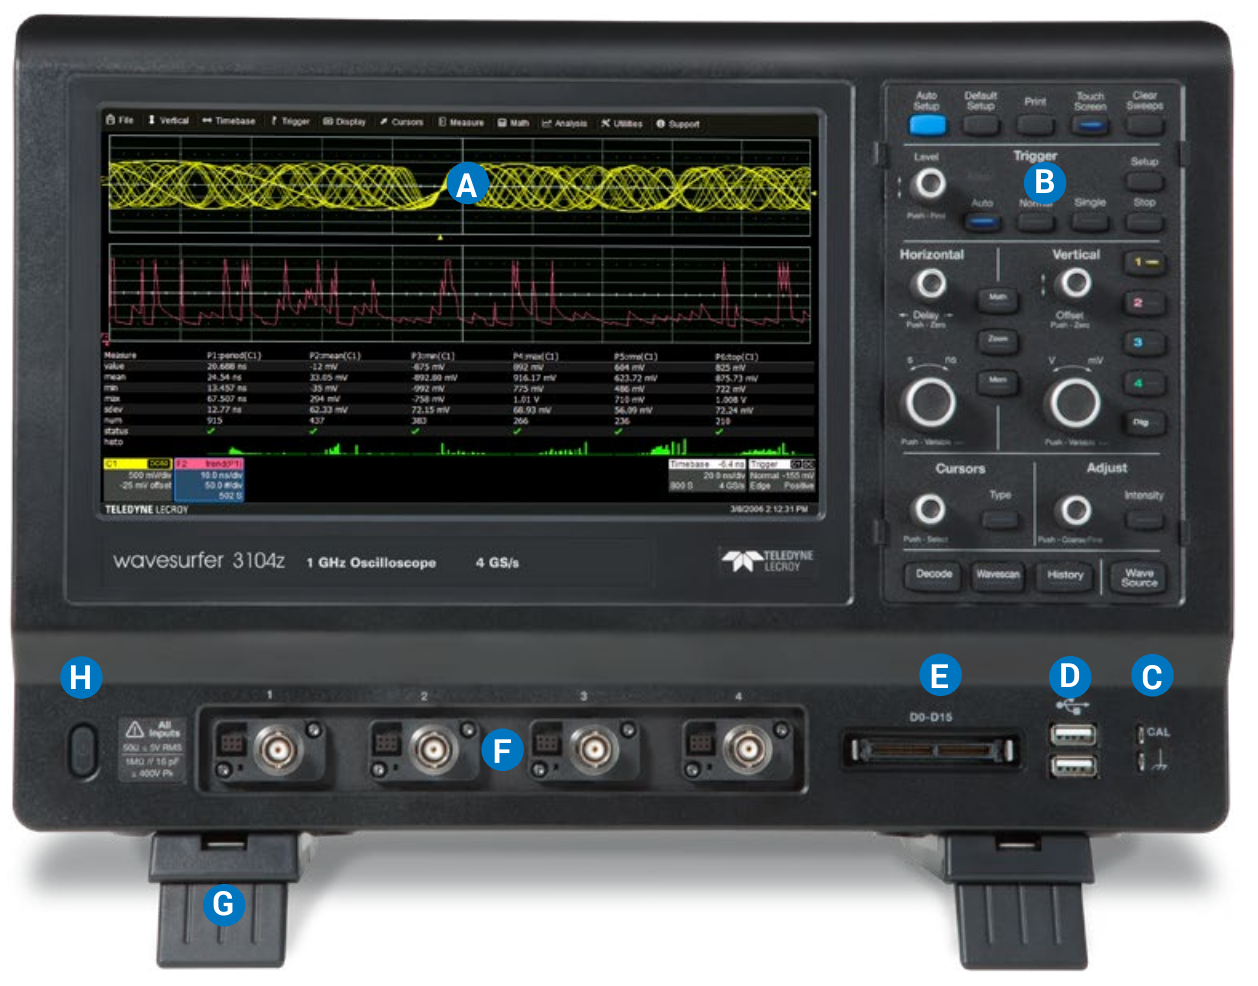
\includegraphics[width=0.9\columnwidth]{lecroy.png}
    \centering
    \caption{View of the front of the oscilloscope from the LeCroy WaveSurfer
             3000z Manual. The following components are labeled: (A) Touch
             screen display, which includes a signal reading, trigger level
             indicator, and setup dialog (B) Front panel, which includes the
             knobs to adjust the offset and voltage per division (C) Ground and
             calibration tunnels (D) USB 2.0 ports (E) Mixed signal interface
             (F) Channel inputs (G) Rotating / tilting feet (H) Power button}
\end{figure}

\subsection{Waveform Analysis Program}

The resulting waveform from the oscilloscope can be ported over to a computer
for data analysis. To graph the data and calculate the lifetimes from our
observations, we wrote a program in Python 3 to extract the lifetime from each
double event recorded, plot a histogram of the data, and calculate the
mean lifetime.

The software uses the popular plotting library \verb|matplotlib| for visualizing
all the data, including the waveform and the histogram. As shown below, the
function \verb|plot_lifetime| instantiates a list of all the relevant filenames
that the program will parse through to extract the muon lifetime. It calls
the function \verb|read_waveform_data|, which simply scans all the points and
compares it to the given threshold value to find the interval between the two
recorded signals. After compiling a list of all the lifetimes, the program
invokes \verb|matplotlib| to bin the results into 10 bins and displays the
histogram to the user.

\begin{lstlisting}[language=Python]
def plot_lifetime(data_path):
    fnames = [os.path.join(data_path, f)
        for f in os.listdir(data_path)
        if os.path.isfile(
            os.path.join(data_path, f)
    )]

    lifetimes = []
    for fn in tqdm(fnames):
        res_x, res_y =
            read_waveform_data(fn)
        lifetimes.append(
            1e6 * find_distance(
                res_x, res_y
        ))
    
    ...

    fig.tight_layout()
    plt.show()

    return avg(lifetimes)
\end{lstlisting}

Using this histogram, we can then manually compile and fit the graph to an
exponential distribution for further analysis. The exponential model is fitted
using \verb|scipy|, which is a scientific computing library for Python, and
error bars representing one standard deviation of uncertainty are also plotted
on the histogram, as shown in Figure 2. The entire software codebase is
available on GitHub.\cite{Yu2020}

\section{Results}

Over the course of approximately 36 hours and 18 minutes, we collected a total
of 1000 double events for analysis. From our calculations, we determined a mean
muon lifetime prior to corrections of $ 2.4158 \pm 0.0764 \mu s$. See Figure 2
for a histogram of the muon lifetimes with 10 bins.

We perform two corrections. The first accounts for accidental doubles, which
are two unrelated events that occur within the same window. The accidental
doubles rate $D_{acc}$ can be calculated using the singles rate $R$ multiplied
by the probability of two events, $E1$ and $E2$ occuring within the same window:
\begin{align}
    D_{acc} = R * P[E1 | E2] = R * R *\nabla t = R^2 \nabla t
\end{align}
where $\nabla t$ is the width of the window. The singles rate is displayed on
the counter and observed to be $9.0185 \mu s^{-1}$. Then the corrected muon
doubles rate, also known as the true doubles rate $D_\mu$, is calculated by subtracting
the total doubles rate from the accidental one.
\begin{align}
    D_\mu = D - D_{acc}
\end{align}
We can find the total doubles rate by dividing the number of events we collected
over the total sampling interval.
Using this, we can calculate the background-corrected mean muon lifetime $T_\mu$ as the
following:
\begin{align}
    D_\mu T_\mu = DT - D_{acc}T_{acc}\\
    T_\mu = \frac{DT - D_{acc}T_{acc}}{D_\mu}
\end{align}
where $T$ is the measured muon lifetime and $T_acc$ can be found by taking the
median time of the window. Using our measured mean muon lifetime, we find that
the background-corrected mean muon lifetime is $2.1037 \mu s$.

For our second correction, we account for the finite window size bias. Since
the interval is finite, we have filtered out muons that decay either very
quickly or very slowly. Although rare, these values can disproportionately
affect the mean. We can find the correction factor $k$ by taking the ratio of
the expectation of the characteristic lifetime, which can be approximated using
the expectation of the exponential distribution, to the expectation of the
average experimental muon lifetime:
\begin{align}
    k = \frac{\int_0^\infty t e^{-t / T_\mu}}{\int_{t_0}^{t_1} e^{-t / T_\mu}}
\end{align}
where $t_0$ and $t_1$ are the start and end of the window. This correction
factor is calculated to be $1.0569$, which we multiply by our result from the
first correction to get the unbiased, background-corrected mean muon lifetime
of $2.2234 \mu s \pm 0.0764 \mu s$.

\begin{figure}
    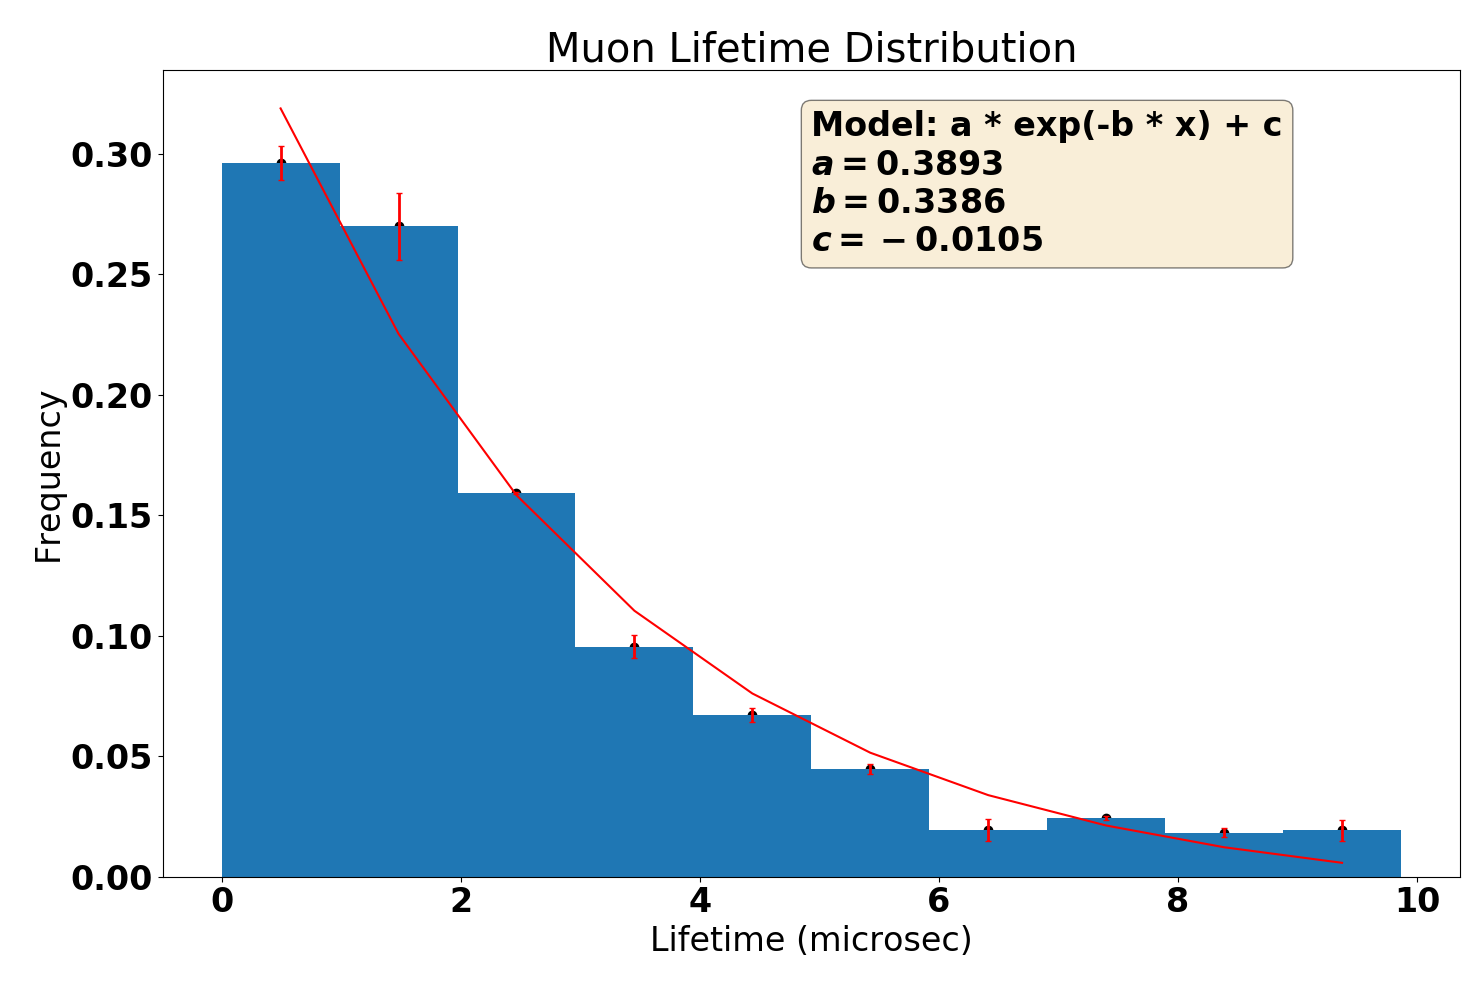
\includegraphics[width=0.9\columnwidth]{hist.png}
    \centering
    \caption{Histogram of the muon lifetimes observed with a trigger interval
             of $[200ns,10 \mu s]$. The number of bins used is 10, and an
             exponential decay model is fitted to the curve, with parameters
             shown in the yellow box. The mean muon lifetime can be found by
             taking the reciprocal of the parameter $b$. See the appendix for
             the expanded figure including histograms using 20 and 30 bins.}
\end{figure}

\section{Discussion}

Our findings determined a mean muon lifetime within about $4.7\%$
of the accepted value. We can explain this error in a number of ways. First,
it is possible for pile-ups to occur when a muon is waiting in the scintillator
to decay that another stray particle may enter and "pre-empt" the muon.
The rate of pile-up events $D_{pu}$ can be calculated as the doubles rate
multiplied by the probability that a singles event will occur in the time
$\delta t$ between the two events of the double. We can then take the
worst-case scenario for long-lived events with $\delta t = 10 \mu s$:
\begin{align}
    D_pu \leq D R \delta t \approx 6.099 * 10^{-11}
\end{align}
Since this is an extremely small number, even a larger number of pile-up
events would drastically affect the results of the calculation, so we determined
that it is not a significant correction needed to be applied. However, since
the accepted value was determined using much more accurate experimental setups,
it is possible for the difference between mean lifetimes to be attributed in
part to pile-up events.

Another method of further reducing this error in future work
is taking additional data. By increasing the number of events collected, we
could arrive at a better fit for the exponential model.
Additional measurements can also be done to find the total cosmic ray rate to
see if the value aligns with our expectation to verify our experimental setup.
This would involve turning off the interval trigger and recording as many
samples as possible. With this method, we could reduce the error in our measured
values, including $R$, to prevent error propagation.

In our second analysis method, we histogram the data by choosing a bin size of
10 and fitting the exponential decay model to the plot. The results produce a
mean muon lifetime, which is found by taking $\frac{1}{b}$, to be $2.95 \mu s$.
This value has a significantly large error compared to the accepted value, which
indicates that there are errors within our histogram method. One potential
source of error that could be fixed is subtracting the background from each bin
to avoid counting accidental events. We could also improve the precision by
weighting the frequencies by the errors to have the exponential decay model
fit better relative to the uncertainty in the data.

Looking at the histogram produced, it is possible to see that a potential source
of error can come from the $[1 \mu s, 2 \mu s]$ bucket, which deviates further
from the best-fit than other points. This could be a result of an error in the
experimental apparatus, which, as described earlier, could be verified by
finding the total cosmic ray rate and calculating the expectation to see if
the results match with our expectations. Another source of error could be the
inherent randomness in the data collected, which is likely since the decay of
the muons is a probabilistic event that becomes more apparent over time.
Although we can never eliminate randomness, it can be reduced with additional
data-taking or repeated trials.

\section{Conclusion}

The unbiased, background-corrected mean muon lifetime determined is
$2.2234 \mu s \pm 0.0764 \mu s$. Further corrections could be made to account
for error propagation in measured values from the experimental devices as well
as the sample size. The histogram produced demonstrates the expected
exponential decay behavior of the muon lifetimes collected. Although the data
collection experiment is somewhat simple, understanding the muon's behavior
has allowed for verification of other physical phenomena. For instance, the
Rossi-Hall experiment verified the relativistic effects of time dilation by
calculating the then-accepted value for the muon lifetime. \cite{PhysRev.59.223}

Similarly, the determination of an extremely accurate value for the mean muon
lifetime also gives the most precise value for the Fermi coupling constant,
which is central to explaining beta decay as proposed by Enrico Fermi in 1933.
Recent developments have also explored the possibility of creating a muon collider,
which could succeed the Large Hadron Collider and offer a 10-fold increase in
energy for the creation of new particles. Understanding the behavior and lifetime
of muons would allow scientists to create muon beams with significantly high
luminosity. Due to their penetrative nature, muons also have other useful
applications that take advantage of our knowledge of muon behavior, including
studying the atomic structures of materials, catalyzing fusion, and elucidate
extremely dense materials that X-rays cannot penetrate.\cite{bross}

\appendix

\section*{Appendix}

The following is the lab instruction sheet provided by Professor May for the
lab for reference: \url{http://www.columbia.edu/~mm21/exp_files/muon.pdf}.
We also used the linked sheet for determining which corrections to make during
the experiment: \url{http://www.columbia.edu/~mm21/exp_files/muoncorr.pdf}

\onecolumngrid

\begin{figure}
    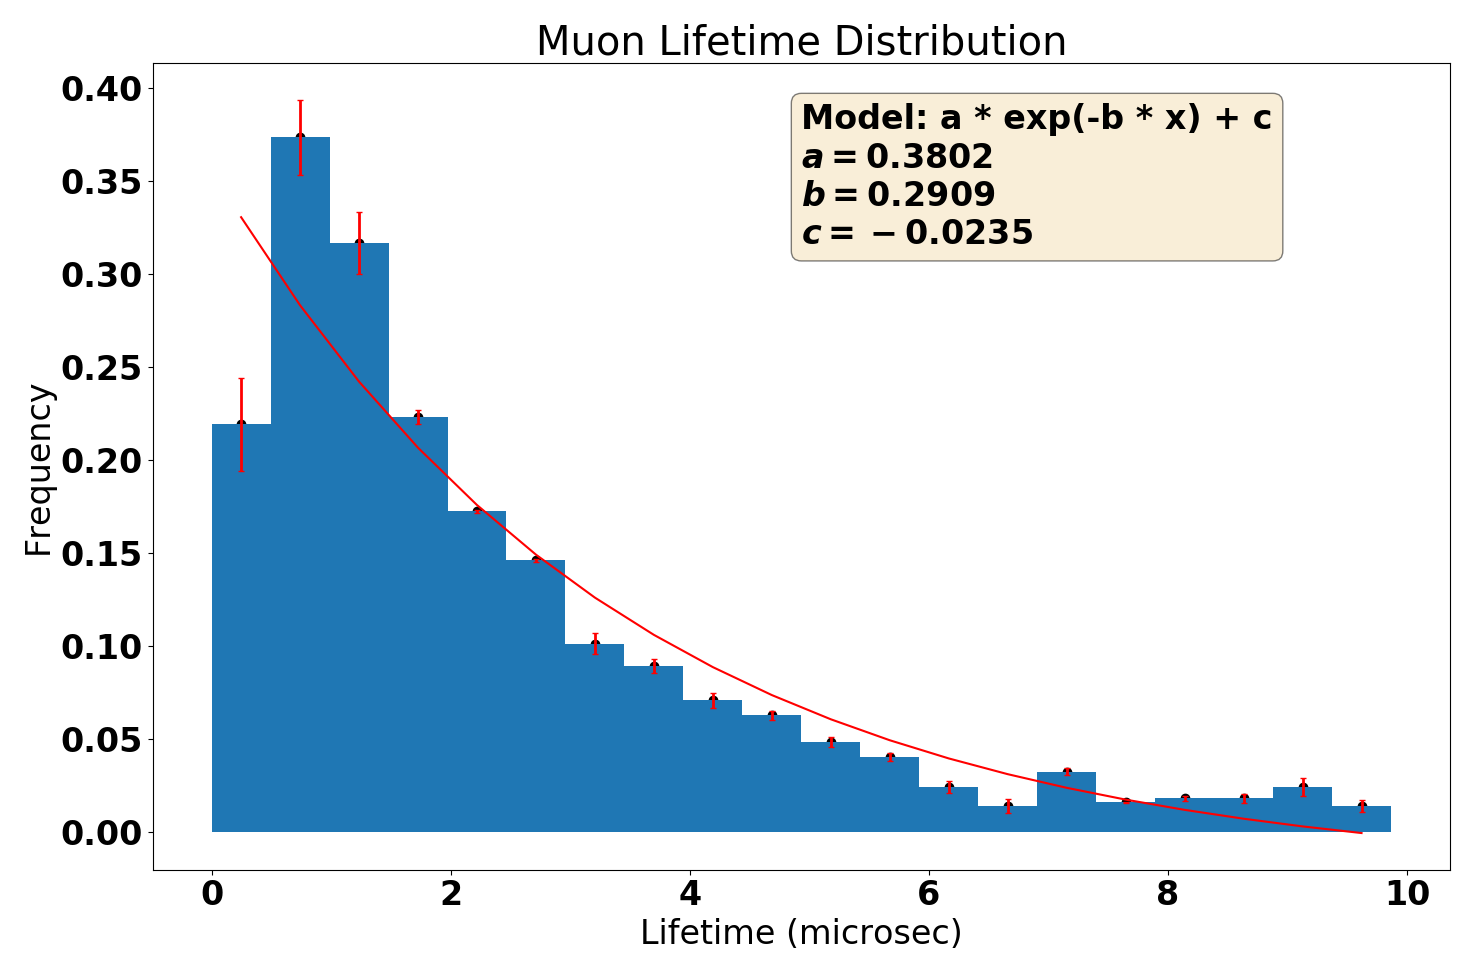
\includegraphics[width=0.4\columnwidth]{hist20.png}
    \centering
    \caption{Histogram of the muon lifetimes observed with a trigger interval
             of $[200ns,10 \mu s]$. The number of bins used is 20, and an
             exponential decay model is fitted to the curve, with parameters
             shown in the yellow box.}
\end{figure}

\begin{figure}
    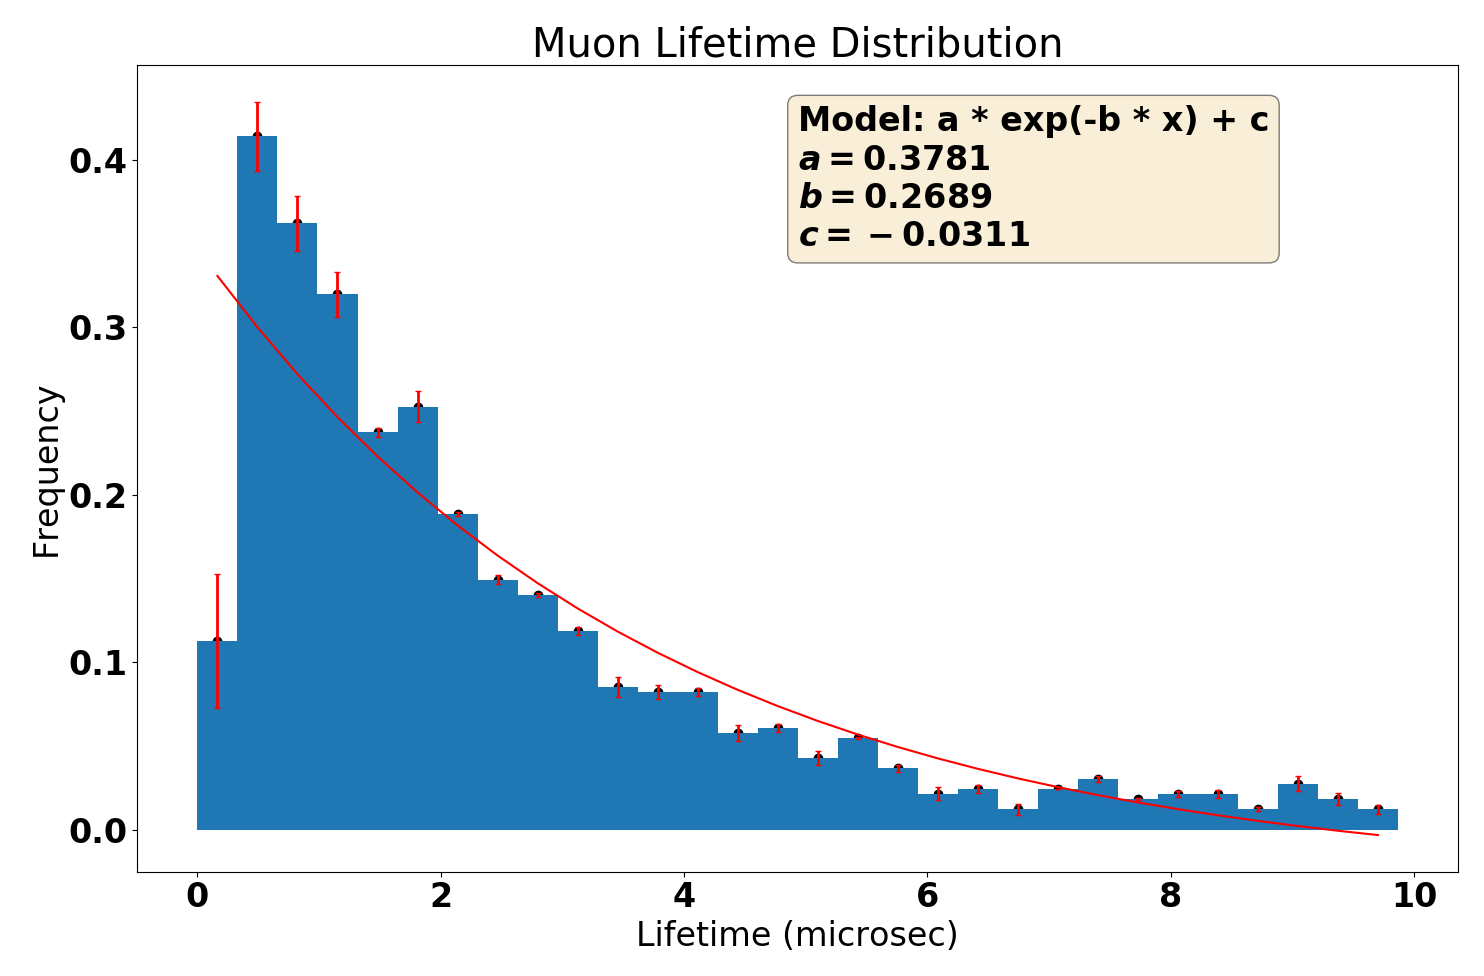
\includegraphics[width=0.4\columnwidth]{hist30.png}
    \centering
    \caption{Histogram of the muon lifetimes observed with a trigger interval
             of $[200ns,10 \mu s]$. The number of bins used is 30, and an
             exponential decay model is fitted to the curve, with parameters
             shown in the yellow box.}
\end{figure}

\bibliography{biblio}

\end{document}
